\documentclass[10pt]{article}
\usepackage[a4paper,margin=2.0cm]{geometry}
\usepackage[T1]{fontenc}
\usepackage{lmodern}
\usepackage{microtype}
\usepackage{amsmath}
\usepackage{booktabs}
\usepackage{graphicx}
\usepackage{caption}
\usepackage{float}
\usepackage[hidelinks]{hyperref}
\graphicspath{{figures/}}
\setlength{\parskip}{0.45em}
\setlength{\parindent}{0pt}
\captionsetup{font=small,labelfont=bf}

\title{\vspace{-1.6em}Ablation of the leaf budget $B$ of BudgetLeafAlias:\\ quality, cost and GPU cache}
\author{}
\date{\vspace{-2.4em}}

\begin{document}
\maketitle
\vspace{-1.0em}

\textbf{Summary.} We swept the leaf budget $B$ of BudgetLeafAlias from 16 to 16000 leaves in all five scenes and over a wide range of light samples per pixel. Where the light is spread over the emitter (Rover, Cinema, Phone), quality is nearly independent of $B$: from 1000 leaves on, every budget is within about 4\% of $B=4000$, mostly within the noise of the measurement. Where the light is concentrated in small regions (Fireplace, Convergence), the error falls steeply up to a few thousand leaves and then levels off: at $B=16$ it is up to 1.6 times that of $B=4000$, at $B=1000$ up to 1.07 times, while $B=16000$ improves on $B=4000$ by only 1--4\%. On the cost side, the sampling structure of $B=4000$ takes 75\,KB and stays in the first-level cache of the GPU; larger budgets exceed it, and sampling becomes 25--29\% slower from 1000 to 16000 leaves in every scene (Section~3), while the per-texel 2D CDF and per-pixel alias table take 2 to 10 times as long. $B=4000$ sits at the knee of both curves.

\section*{1\quad Setup}

\emph{Quality.} BudgetLeafAlias with $B$ = 16, 64, 250, 1000, 2000, 4000, 8000 and 16000, in the five scenes of the paper, three frames per scene, rendered with the engine's own sampler in our GPU path tracer. We vary the number of light samples per pixel, $\text{spp} = $ samples per pixel $\times$ light samples per shading point: the light samples per shading point are fixed per scene (16 in Rover, 8 in Cinema, 4 in Fireplace, 6 in Phone and 3 in Convergence), and the samples per pixel range from 1 to 128, so that spp covers two orders of magnitude in each scene (e.g.\ 8 to 1024 in Cinema). Each configuration is captured six times with independent random numbers, and we report the RMSE against a converged reference of each frame, averaged over captures and frames. The 2D CDF and the per-pixel alias table are rendered on the same grid as baselines.

\emph{Cost.} A dedicated compute pass draws light samples with each sampler, without ray intersection or shading, with one thread per pixel of a $1920\times1080$ frame and 128 light samples per thread. Its dispatch alone is timed with GPU timestamps. Each configuration (scene, sampler and $B$) is run as a separate process, the median over 60 frames is kept, and the runs are repeated in three rounds, each in a shuffled order, so that variations of the GPU clock between processes affect all configurations alike. We report the median of the three runs: an occasional run lands in a faster clock state, always on the fast side, and the median discards it. We use 128 samples per thread because shorter dispatches leave the GPU idle between frames, and its clock then varies between runs by up to 30\%, more than the differences we want to measure.

\emph{Cache.} A pointer-chase benchmark and a per-sample cost benchmark (Section~4) relate these costs to the cache levels of the GPU. All measurements on one RTX 4080 SUPER.

\section*{2\quad Quality against the number of leaves}

\begin{figure}[H]
\centering
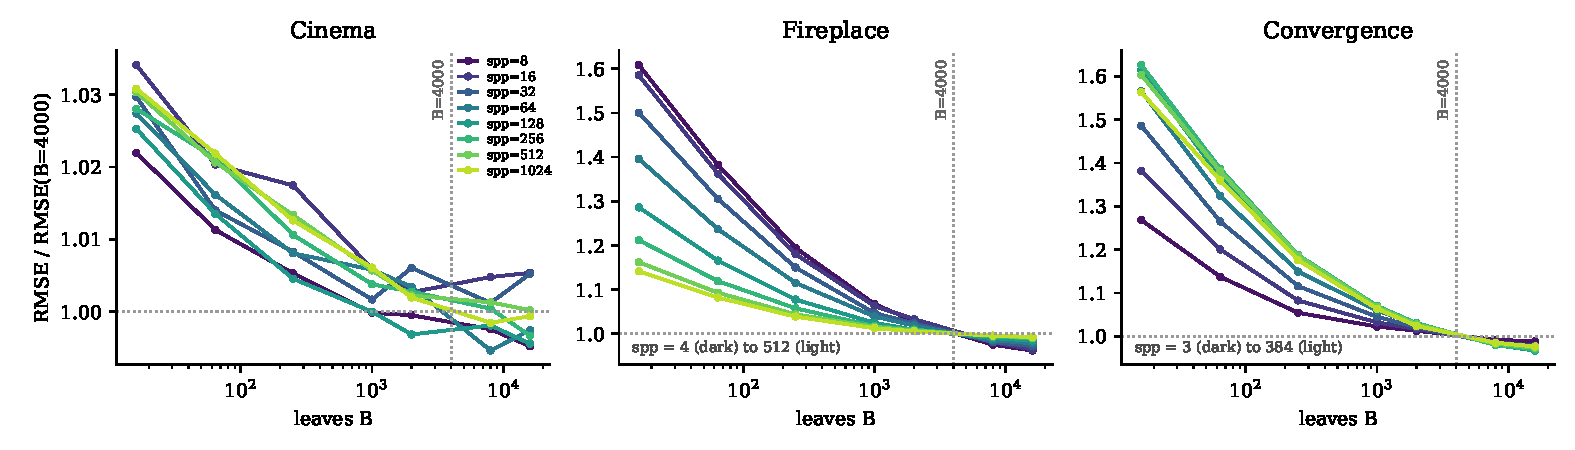
\includegraphics[width=\linewidth]{final_relative_cinema_fireplace_convergence.pdf}
\caption{RMSE against the converged reference, divided by the RMSE of $B=4000$ at the same number of light samples per pixel (spp), as a function of the leaf budget $B$. Each curve is one spp; Cinema's values are in the legend, and the other scenes use the same color order from their lowest to their highest spp. Values above 1 mean more error than $B=4000$.}
\label{fig:quality}
\end{figure}

Figure~\ref{fig:quality} shows the error of each budget relative to $B=4000$ at equal samples, so that only the quality of the leaf density is compared. Two behaviors appear, depending on how the light is distributed over the emitter.

In Cinema, light is spread over most of the screen, and a coarse partition already matches it: even 16 leaves are within 2--3.5\% of $B=4000$, from 1000 leaves on every budget is within 0.6\%, and the curves for different spp overlap. Rover and Phone, whose light is also spread out, behave in the same way (not shown): from 1000 leaves on, every budget is within 2--4\% of $B=4000$, and the differences are mostly within the noise of the measurement.

In Fireplace (flames) and Convergence (lamps), most of the energy sits in small regions that the partition must resolve, and the error falls steeply with $B$ before levelling off. In Convergence, 16 leaves give up to 1.63 times the error of $B=4000$, 250 leaves up to 1.19 times, and 1000 leaves up to 1.07 times, while doubling or quadrupling the budget beyond 4000 improves the error by only 1--3\%. This penalty grows with spp and stabilizes from about 24 spp on. We attribute the smaller differences at the lowest sample counts to the comparison being made on display-referred images clamped to $[0,1]$: at very low spp many noisy pixels are clamped, which limits the error of every budget alike and compresses the ratios. In Fireplace, the penalty of small budgets is largest at low spp (1.61 times at 16 leaves and 4 spp) and decreases with spp (1.14 times at 512 spp). In this scene the error of every sampler, including the 2D CDF, decreases more slowly than $1/\sqrt{\text{spp}}$, which indicates an error component common to all samplers that does not decrease with the number of samples and compresses the ratios at high spp. \textbf{In both scenes, the gain from 4000 to 16000 leaves stays between 1 and 4\% at every spp.}

\section*{3\quad Cost of sampling against the number of leaves}

\begin{table}[H]
\centering\small
\setlength{\tabcolsep}{5pt}
\begin{tabular}{lccccc|cc}
\toprule
& \multicolumn{5}{c|}{BudgetLeafAlias, $B$ =} & Per-pixel & \\
& 1000 & 2000 & 4000 & 8000 & 16000 & alias & 2D CDF \\
\midrule
Rover & 11.5 & 12.1 & 13.8 & 13.7 & 14.7 & 27.6 & 118.3 \\
Cinema & 11.5 & 12.0 & 13.2 & 14.4 & 14.8 & 30.2 & 110.0 \\
Fireplace & 11.5 & 12.1 & 13.2 & 14.0 & 14.5 & 75.7 & 63.8 \\
Phone & 11.5 & 12.1 & 13.3 & 14.2 & 14.6 & 22.9 & 114.8 \\
Convergence & 11.7 & 12.1 & 13.1 & 14.1 & 14.7 & 69.9 & 62.1 \\
\midrule
Structure size & 19\,KB & 38\,KB & 75\,KB & 150\,KB & 300\,KB & 41.5--166\,MB & 16.6--66\,MB \\
\bottomrule
\end{tabular}
\caption{GPU time of light sampling alone, without ray tracing or shading, for one $1920\times1080$ frame at 128 light samples per pixel, in milliseconds (median of three runs), and size of each sampling structure. Rover, Cinema and Phone have 1080p emitters; Fireplace and Convergence have 4K emitters.}
\label{tab:sampling}
\end{table}

Table~\ref{tab:sampling} reports the time spent drawing light samples for a full-HD frame, isolated from the rest of the path tracer. The cost of BudgetLeafAlias depends on the leaf budget but hardly on the scene: at $B=1000$ a frame's sampling takes 11.5--11.7\,ms in all five scenes, and it rises steadily with $B$, by 4--5\% at $B=2000$, 12--20\% at $B=4000$, 19--25\% at $B=8000$ and 25--29\% at $B=16000$. The structure grows by about 19 bytes per leaf, from 19\,KB at $B=1000$ to 75\,KB at $B=4000$, 150\,KB at $B=8000$ and 300\,KB at $B=16000$, so the larger budgets no longer fit in the first-level cache of the GPU (128--192\,KB, Section~4), and the cost keeps rising beyond that limit. The per-texel structures are far more expensive: the per-pixel alias table takes 2.0--2.6 times the time of $B=1000$ with 1080p emitters and 6.0--6.6 times with 4K emitters, and the 2D CDF 9.6--10.3 times and 5.3--5.5 times, respectively; Section~4 explains why the per-pixel alias table, despite its $O(1)$ sampling, becomes the slower of the two at 4K. In a full frame of our path tracer, where light sampling is only one of many costs, the difference between budgets is diluted: at 256 light samples per pixel in Cinema, the frame takes 235\,ms at $B=1000$, 240\,ms at $B=4000$ and 241\,ms at $B=16000$, against 284\,ms with the per-pixel alias table and 584\,ms with the 2D CDF.

\section*{4\quad Cost and GPU cache}

\begin{figure}[!ht]
\centering
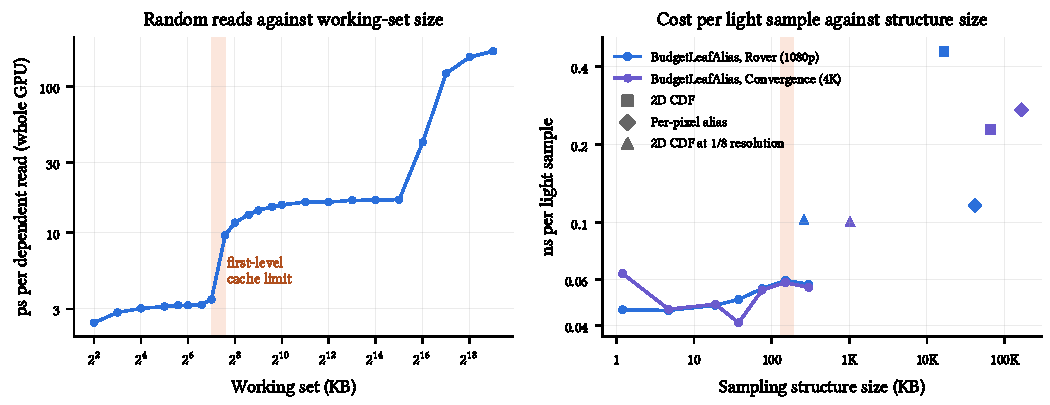
\includegraphics[width=\linewidth]{gpu_cost.pdf}
\caption{Left: latency of dependent random reads against the size of the data being read, on the GPU (pointer chase, aggregate over the whole GPU). Right: measured cost of one light sample against the size of the sampling structure: BudgetLeafAlias from 64 to 16000 leaves (lines), and the 2D CDF, per-pixel alias and a 2D CDF built at one eighth of the resolution (markers), in Rover (1080p, blue) and Convergence (4K, purple). Shaded: the first-level cache limit, 128--192\,KB.}
\label{fig:cache}
\end{figure}

We relate the cost of sampling to the cache levels of the GPU with two benchmarks. First, a pointer-chase benchmark reads memory in a chain of dependent random accesses and reports the time per read as the working set grows from 4\,KB to 512\,MB; this exposes the cache levels of the GPU (Figure~\ref{fig:cache}, left). Second, a dedicated compute pass draws 8.4 million light samples per dispatch with each sampler ($1024\times1024$ threads, 8 samples each), with no ray intersection or shading. In both benchmarks we time the dispatch alone with GPU timestamps, take the median over the frames, and divide it by the total number of reads or samples in the dispatch ($512\times512$ threads of 128 reads each for the pointer chase, 70 frames; for the sampling pass, the median of three repeated runs of 130 frames each). The reported times are therefore throughputs of the whole GPU, not the latency of an individual sample: thousands of threads run concurrently and hide part of each other's memory latency, so a single sample takes far longer than its share of the dispatch time. We run it for BudgetLeafAlias at every leaf budget, whose structure takes about 19 bytes per leaf (75\,KB at $B=4000$), and for the 2D CDF and per-pixel alias, whose structures cover every texel (16.6 and 41.5\,MB at 1080p, 66 and 166\,MB at 4K), as well as for a 2D CDF built at one eighth of the resolution (260\,KB and 1\,MB). Figure~\ref{fig:cache} (right) plots each sampler's cost against the size of its structure.

A GPU reads memory through a hierarchy: a small first-level (L1) cache in each streaming multiprocessor, a second-level (L2) cache shared by the whole chip (64\,MB on our GPU), and the device memory (DRAM). A read served by a cache is a \emph{hit}; a read that must go to the next level is a \emph{miss}, and its latency grows by roughly an order of magnitude at each level, reaching hundreds of clock cycles for DRAM. When the address of a read depends on the value returned by a previous one (a \emph{dependent read}), these latencies add up, because the second read cannot start before the first completes. The pointer-chase benchmark measures exactly this case, and shows a sharp limit (Figure~\ref{fig:cache}, left): dependent random reads cost about 3\,ps, in aggregate over the whole GPU, while the data fits in L1, three times as much (9.6\,ps) once the working set exceeds 128--192\,KB, and tens of times more beyond L2. The sampling cost follows the same limit (Figure~\ref{fig:cache}, right). The 2D CDF and the per-pixel alias table store one entry per texel, tens of megabytes that remain far outside L1, and cost 0.12--0.46\,ns per sample, whereas BudgetLeafAlias at $B=4000$ costs 0.055\,ns, 2 to 8 times less. The 2D CDF built at one eighth of the resolution, whose structure still takes 260\,KB to 1\,MB, falls in between at 0.10\,ns: the same algorithm becomes 2 to 4.5 times cheaper merely by shrinking its structure.

Within BudgetLeafAlias the cost per sample rises far less than the latency of a single dependent read. From 4.7 to 38\,KB a sample costs 0.041--0.050\,ns; around the L1 limit (75--150\,KB) it rises to 0.055--0.060\,ns, 20--30\% more, and remains there at 300\,KB. A sample performs only one or two dependent reads among other independent work, so the GPU hides part of their latency by running other threads, and the leaves sampled most often are those where the light is, so most of them likely remain cached even when the whole structure no longer fits. At 75\,KB, $B=4000$ uses most of the L1 capacity without exceeding it, whereas doubling it to 8000 leaves (150\,KB) reaches the limit.

The sampling benchmark also shows that the per-pixel alias table, despite its $O(1)$ sampling, is not cheaper than the 2D CDF, whose sampling is $O(\log n)$. The benchmark times the whole sampling call: choosing the texel, reading its weight, converting the density to solid angle and reading the radiance at the sampled point. The last three steps are the same for every sampler; only the choice of the texel differs, and its cost is determined by where the data is read from rather than by the number of operations. The per-pixel alias table performs two dependent reads per sample. The first random number selects one of its buckets uniformly, independently of the texels' brightness, and the sampler reads that bucket (16 bytes); the selected texel's weight, needed to evaluate the density, is then read at a second, unrelated location. Because these addresses are spread uniformly over the whole structure, 41.5\,MB at 1080p and 166\,MB at 4K, almost every read misses L1. At 1080p the structure largely fits in L2, but at 4K it exceeds it and most reads are served from DRAM. The arithmetic is identical in both cases, yet the cost per sample more than doubles, from 0.116\,ns in Rover to 0.272\,ns in Convergence.

The 2D CDF draws a sample by inverting two cumulative distribution functions: the \emph{marginal} CDF over the image rows, which selects a row with probability proportional to its total luminance, and the \emph{conditional} CDF of that row, which selects a texel within it. Each inversion is a binary search of about 11--12 steps, so a sample requires about 24 dependent reads, an order of magnitude more than the alias table. These reads, however, are mostly cache hits. The marginal CDF has only $H+1$ entries (4--9\,KB) and stays permanently in L1. Each conditional search is confined to a single row of $W+1$ entries (8--15\,KB), and since rows are selected in proportion to their luminance, the accesses concentrate on the few bright rows, which therefore remain in cache. This locality also explains why the 2D CDF is cheaper in Convergence (0.229\,ns), where the light is concentrated in a few lamps and a few rows receive most of the samples, than in Rover (0.459\,ns), where the light, and hence the accesses, are spread over many rows. The comparison is thus between about 24 mostly cached reads and 2 reads that nearly always miss, and since a single DRAM access costs as much as dozens of cache hits, at 4K the per-pixel alias table is even slower than the 2D CDF. \textbf{The constant operation count of the alias method translates into a low cost only when its table resides in cache.} BudgetLeafAlias performs exactly the same two alias reads, but on a 75\,KB table that remains in L1, and costs 0.055\,ns per sample.

\section*{5\quad Conclusions}

The leaf budget $B$ trades quality against cost, and both curves have a knee at a few thousand leaves. On the quality side, emitters with spread-out light are matched by a few hundred leaves, while emitters with concentrated light need a few thousand: below 1000 leaves their error grows quickly, by up to 60\% at 16 leaves, and above 4000 leaves it improves by only 1--4\%. This holds at every number of light samples per pixel we tested, from 3 to 1024. \textbf{On the cost side, the sampling structure grows by about 19 bytes per leaf and stays within the first-level cache of the GPU up to about 4000--8000 leaves; the cost of sampling rises steadily with the number of leaves and keeps rising beyond the cache, for a total of 25--29\% from 1000 to 16000 leaves. $B=4000$ therefore captures nearly all the quality available from the partition while keeping the structure in cache.} It is not a fragile tuning parameter: in quality, any budget between 2000 and 16000 is within 4\% of it in every scene, and devices with less memory can use a smaller budget at the quality cost shown in Figure~\ref{fig:quality}.

\end{document}
